\documentclass[a4paper,12pt]{article}
\usepackage[a4paper,margin=1in,footskip=0.25in]{geometry}
\usepackage[utf8]{inputenc}

% science
\usepackage{amsmath}
\usepackage{array}
\usepackage{siunitx}

% layout
\usepackage{float}
\usepackage{parskip}
\usepackage{graphicx}
\usepackage{longtable}
\usepackage{hyperref}

\usepackage{caption}
\usepackage{subcaption}
\usepackage{wrapfig}
\usepackage{fancyhdr}

% referencing
\usepackage[style=apa]{biblatex}
\addbibresource{azero.bib}
\usepackage{hyperref}


% figures labelings
\usepackage{chngcntr}
\counterwithin{figure}{section}

\renewcommand{\arraystretch}{1.7}
\newcolumntype{P}[1]{>{\raggedright\arraybackslash}p{#1}}
\newcommand{\tptt}{$\times\,$}

% uncertainty
\newcommand{\absun}{\Delta \text{unc}\,}
\newcommand{\relun}{\% \text{unc}\,}

\title{Empirically finding the value of absolute zero using the ideal gas law}

% no author or date
\author{}
\date{\vspace{-8ex}}

% bottom right
\pagestyle{fancy}
\fancyhf{}
\fancyfoot[R]{\thepage}
\fancypagestyle{plain}{%
    \renewcommand{\headrulewidth}{0pt}%
    \fancyhf{}%
    \fancyfoot[R]{\thepage}%
}
%go
\renewcommand{\headrulewidth}{0pt}

\begin{document}

\maketitle

\section{Design}
\subsection{Introduction}
On my Duke of Edinburgh bronze medal trip, we were using butane gas tanks to cook the various dinner each of us has bought. The supervisor --- which happened to be a physics teacher, informed us to be careful with the butane gas tanks. He stated that when heated, they will explode due to the pressure buildup within the cans.

For I often go outdoors and camp overnight, I find this phenomenon both interesting and important --- for my own safety. After some initial research \parencite{lpg}, and flicking through the IB textbook, I stumbled upon a relationship between the temperature and pressure of gases, indicating that the explosion is caused by the increase in the pressure of the butane gas inside the container under temperature changes. Therefore I decided to investigate the relationship between temperature and pressure of gases, which caused me to realize its connection to a fundamental quantity when I extrapolate the regression line.

While I've been told in class that the temperature of absolute zero is not physically reachable and is only useful in calculations, I now have a simple yet powerful procedure that calculates this value. This investigation aims to empirically find the value of absolute zero using the relationship between the temperature and pressure of a sample of air mixture.


\subsection{Research Question}
\begin{quote}
    What is the relationship between the pressure of a sample of air mixture against its temperature under constant container volume and mixture molecular quantity?
\end{quote}

\subsection{Background}
% talk about gases and the ideal gas law
There exists a wide range of chemical reactions that includes a variety of gases as reactants or products. For the sake of stoichiometric analysis, it is heavily desired to be able to model the behavior of gases. To ease the calculations involved with the millions of individual gas particles at the microscopic level, the field of ``kinetic theory of matter'' created a model of the ideal gas with idealistic assumptions that still often resemble real gases.

The five assumptions of an ideal gas are that: (1) the gas molecule collisions are elastic, (2) the volume of the particles is negligible, (3) there exists no intermolecular forces between the particles, (4) the particles of a gas obey Newtonian motion and move with a range of speed and direction \parencite{gas_law}. These assumptions will be helpful in designing my experiment.

With the help of numerous scientists over the span of 400 years, the model of the ideal gas can be summarized in figure \ref{fig:igl}.

\begin{figure}[H]
    \[
    PV = nRT
    \]
    \caption{The Ideal Gas Law}
    \label{fig:igl}
\end{figure}

The law contains the relationships between the four gaseous state quantities, each in their respective standard units: $P$ for Pressure, $V$ for Volume, $n$ for the number of moles, and $T$ for temperature. We are interested in strictly the relationship between temperature and pressure. Thus when extracting from the law, we arrive at the relationship in figure \ref{fig:pt}, where $c$ is the proportionality constant. This relation is also initially discovered by Joseph Louis Gay-Lussac.

\begin{figure}[H]
    \[
    P = cT
    \]
    \caption{Pressure and Temperature relationship}
    \label{fig:pt}
\end{figure}

The relationship showcases that as the temperature of an ideal gas increases, its pressure also increases. This is because pressure measures the average force per unit area of the moving particles in the gas elastically colliding with the walls of the container. For temperature is a measure of the average kinetic energy of the particles, its increase means overall faster-moving particles, causing an average larger force upon the gas container \parencite{pearson}.

% For there is a linear relationship between pressure and temperature, in the case of an ideal gas, I should measure a linear trend when graphing the gas pressure against its temperature, with an intercept of zero when the units are standard (Pascals and Kelvin).%


\begin{wrapfigure}{r}{0.5\textwidth}
    \centering
    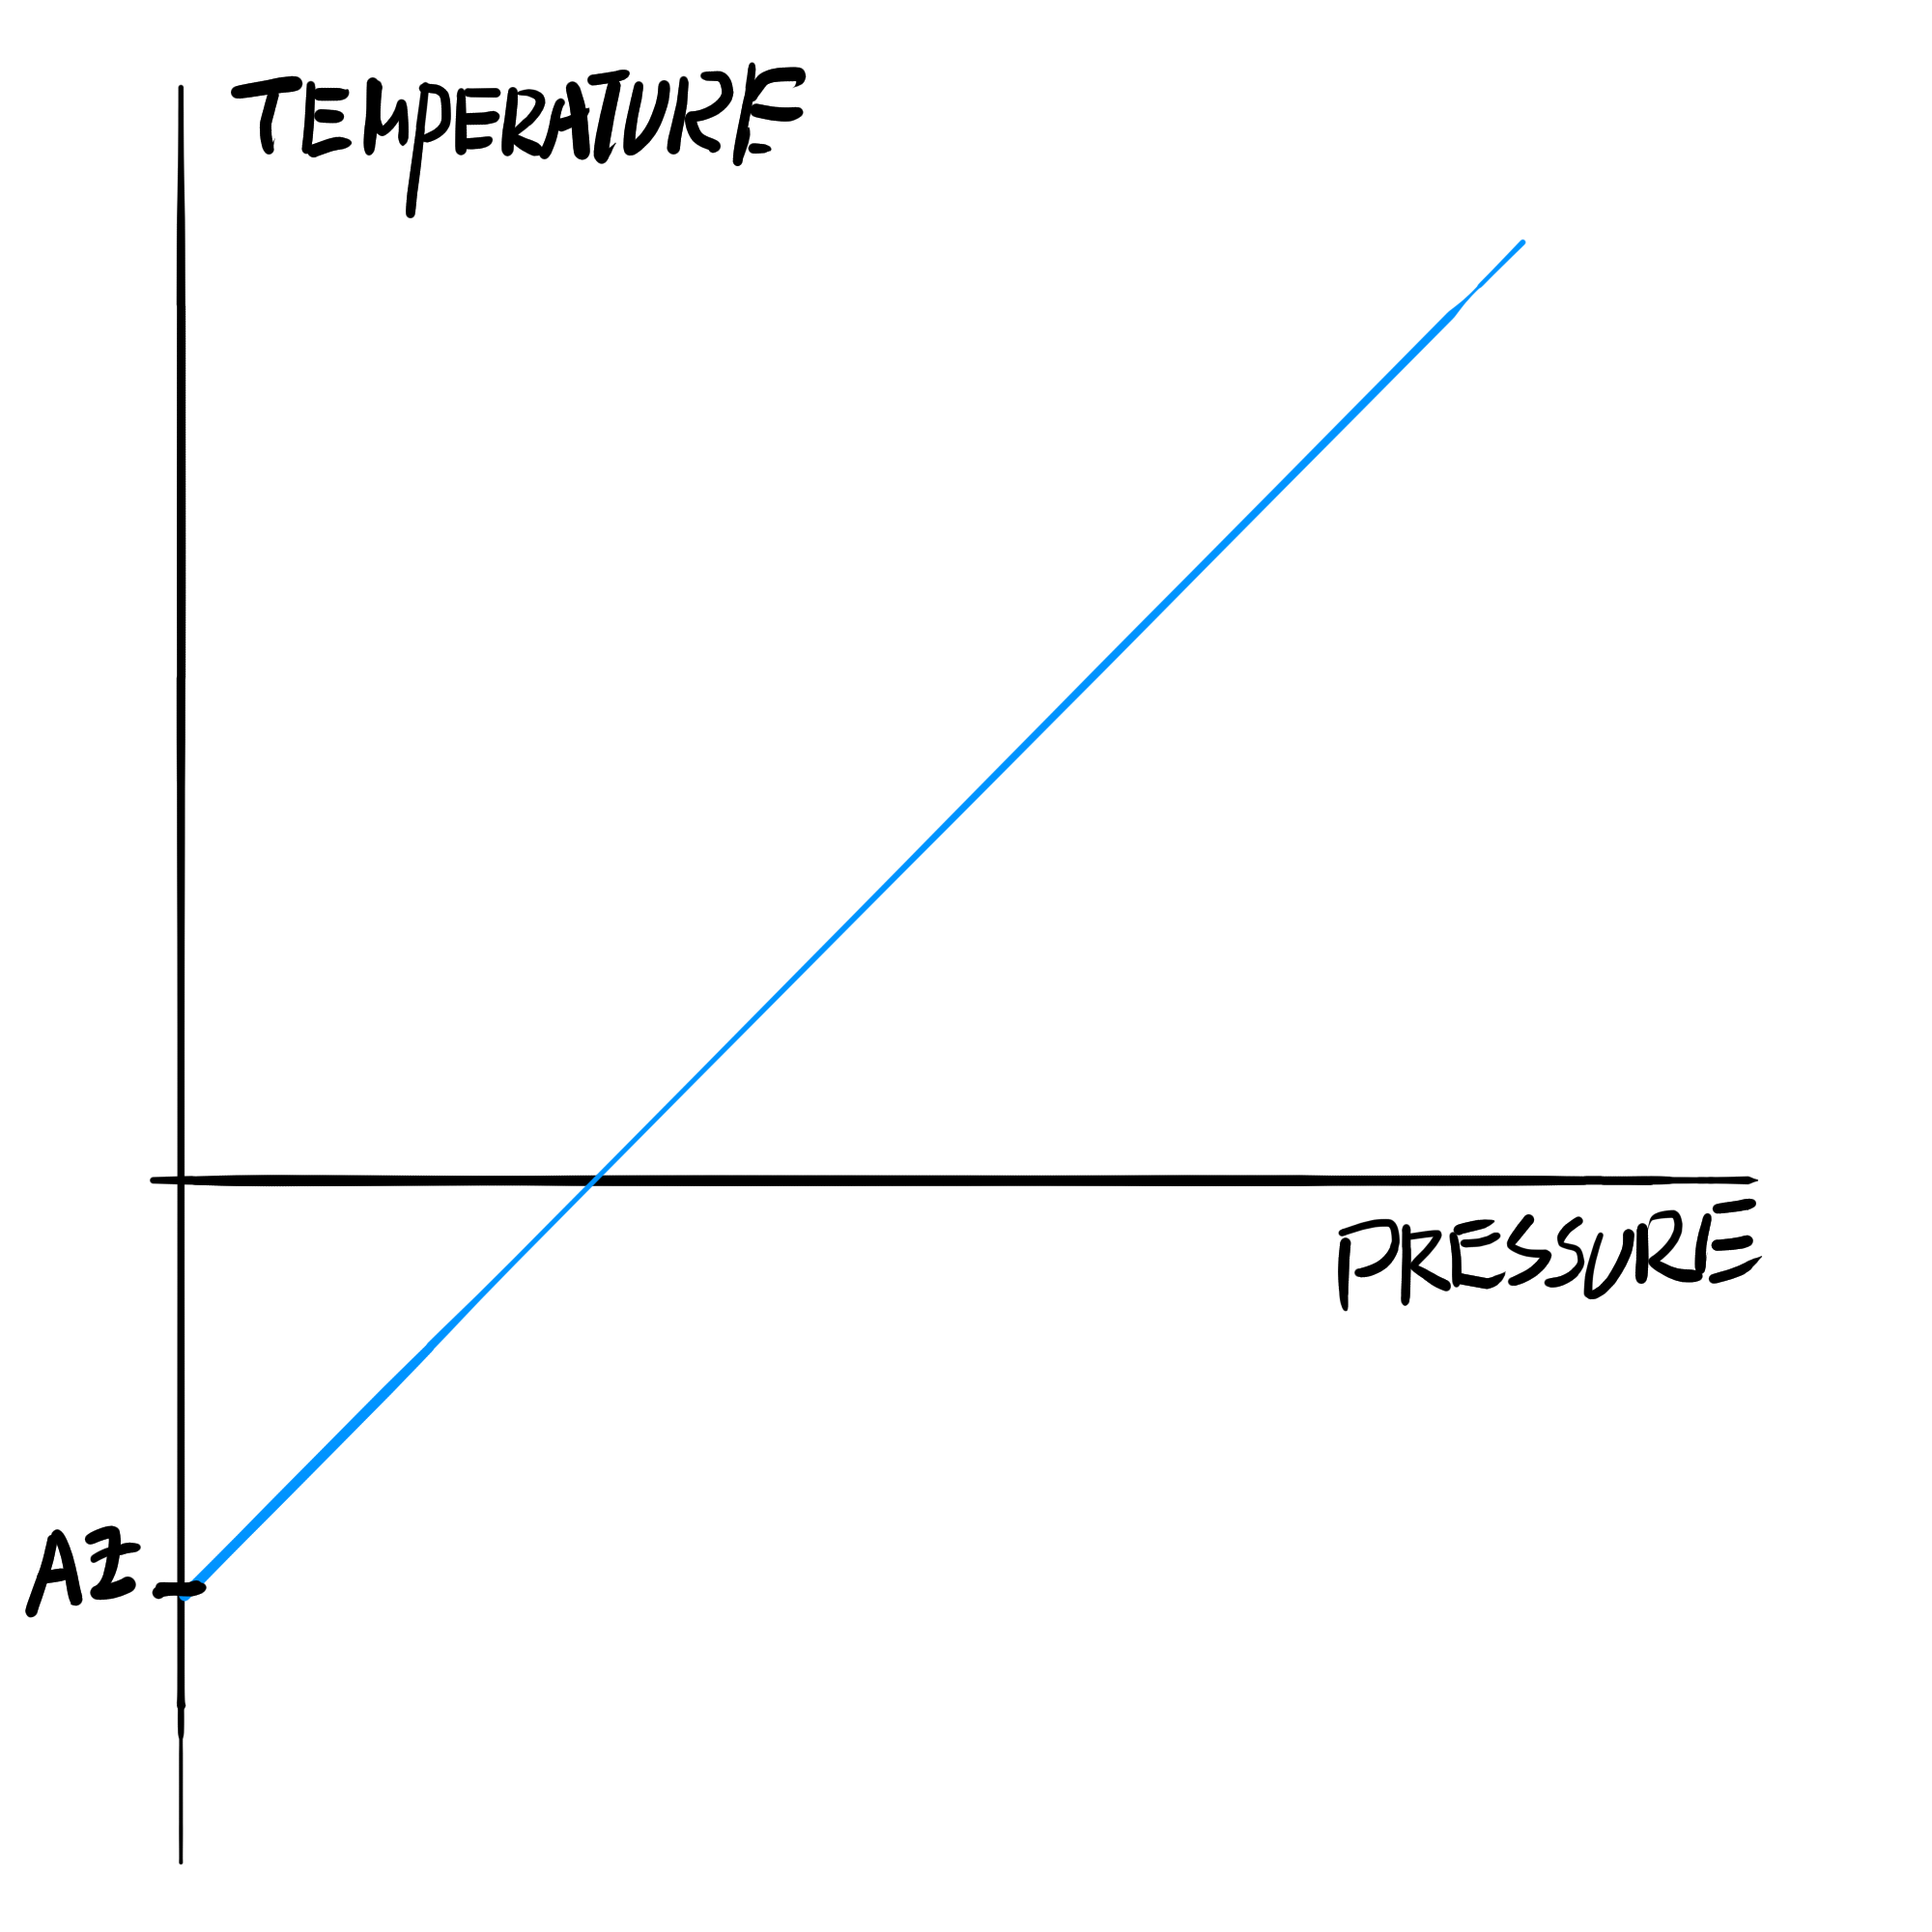
\includegraphics[width=0.37\textwidth]{assets/az.png}
    \caption{Transposed T vs. P graph}
    \label{fig:az}
\end{wrapfigure}

% its connection to the idea of absolute zero
By transposing the two axis (so that it is a Temperature against Pressure graph), extrapolating the linear relationship:
\[
    T = \frac{1}{c}P,
\]
can display an incredible result. The absolute zero is a theoretical measurement of temperature that sets the lower bound of the temperature scale. At the temperature, the velocities of the gas particles are precisely zero, therefore the gas has zero outwards pressure. So the y-intercept (AZ) of the regression line (figure \ref{fig:az}), should be zero when using a standard unit such as Kelvin, and would measure the value of absolute zero in Celsius when the temperature unit is in Celsius.


% https://en.wikipedia.org/wiki/Barometric_formula?oldformat=true
% Additionally, the proportionality constant $k$ can be used to determine the boiling point of water at a range of attitudes. A substance boils when the average kinetic energy of the particles exceeds average kinetic energy of the surrounding air. Macroscopically, this occurs when the pressure of the liquid is higher than the atmospheric pressure. The barometric function $P(h)$ is a mapping between heights and the atmospheric pressure, therefore we can deduce the boiling point


% how I would measure it
% potential source of errors
To test the theory, I have decided to use a pressure probe containing a sample of air mixture dipped in water within a beaker above a bunsen burner, where the temperature of the water is the independent variable and pressure of the air mixture is the dependent variable. The chosen range of temperature is from $20\si{\celsius}$ to $100\si{\celsius}$, for it ensures the widest possible range of temperatures of water (room temperature to boiling point) for regression.

I chose to heat the water up to its boiling point, and waiting for it to cool down to a reasonable temperature of around $65\si{\celsius}$, taking measurements along the way. For the uncertainty of the pressure probe is relatively high, I choose to repeat this experiment a total of 5 times to increase its accuracy.

For the air mixture is transparent to my eye, the gas particles are likely to have minimal size. In combination with the large volume of the container (figure \ref{fig:probe}), the air mixture satisfies most of the assumptions and thus can be modeled with the ideal gas law. Therefore I hypothesize a positive correlation between the temperature and the pressure of the mixture, approximating a linear graph to that of figure \ref{fig:az}.

\subsection{Variables}
\paragraph{Independent Variable}
The temperature of the air mixture in degrees Celsius. This is measured using a digital thermometer in water with uncertainty ($\pm 0.1\si{\celsius}$). The temperature ranges from room temperature to the boiling point of water, from $\approx20\si{\celsius}$ to $ \approx100\si{\celsius}$.

\paragraph{Dependent Variable}
The pressure of the air mixture in PSI. This is measured using a pressure probe (figure \ref{fig:probe}) submerged in 200ml water in a 500ml beaker with uncertainty ($\pm 0.25\text{psi}$). The pressure ranges from $14\text{psi}$ to $19\text{psi}$.

\subsection{Control Variables}

% table here
\begin{longtable}{P{0.2\textwidth}|P{0.35\textwidth}|P{0.35\textwidth}}
Controls & Reason & How\\\hline

Submersion depth of pressure probe & The submersion depth of the probe determines the surface area between the glass container with the heated water. The larger the surface area, the faster the heat conducts from the water to the air mixture, causing a lower than measured temperature inside the probe and creating systematic error in the y-intercept of the pressure vs. temperature relationship & Use a constant volume (200ml) of water and a constant size beaker (500ml) for each experiment. The water should submerge the spherical bulb up to the stem, but not too much as to overflow \\

Interval between measurements & Pressure probe uncertainty means a small change in temperature does not reflect in a change in pressure, frequent measurements will map multiple temperature values to a single pressure value. As temperature rate of change fluctuates throughout the experiment, a random amount of temperature measurements per pressure value. This randomly weights each pressure measurement in the regression process, causing random error in the y-intercept & Use a timer to take measurements every 30 seconds when heating, and every 1 minute when cooling, as to ensure meaningful pressure changes during the intervals \\

Placement of sensors & Contact between the sensors and the beaker will cause systematic error in their measurements & Using clamps to suspend the thermometer and gas pressure probe within the water. (Also avoid direct contact between the sensors) \\

Environmental atmospheric pressure & Changes in the surrounding atmospheric pressure can systemically increase the pressure measurements & Conduct the experiment at the same location for each trial, ideally all within a short time span of a week
\\

Method of measurements & Non-direct viewing of the pressure probe will cause parallax error in the pressure measurements. Guessing dim thermometer readings can create random errors & View the pressure probe upright and direct, prepare a backup thermometer to switch in if the current one becomes dim or hard to read \\
\end{longtable}

\subsection{Materials}

\begin{itemize}
    \item gas pressure measurement probe ($\pm 0.25\si{psi}$) (figure \ref{fig:probe})
    \item 500ml glass beaker with volume markings ($\pm 50\si{ml}$)
    \item 2 $\times$ digital thermometer ($\pm 0.1\si{C}$)
    \item 2 $\times$ retort stands \& clamps
    \item a timer ($\pm 1\si{s}$)
    \item bunsen burner, tripod, gaze mat, and heating mat
    \item lighter
\end{itemize}

\subsection{Method}


\begin{enumerate}
    \item Connect the bunsen burner to the gas output and place it on top of a heating mat on a table, place the tripod on top of the burner with a gaze mat on the tripod. Place the 500ml glass beaker on top of the gaze mat. Setup the two retort stands by attaching the clamps, then fitting the pressure probe and thermometer to each of the clamp. Slowly lower the sensors so that they are inside the glass beaker. Check the setup matches figure \ref{fig:setup}, or figure \ref{fig:setupdrawn}.
    \item Lift the two clamps holding the sensors. Fill the glass beaker with tap water, stop at 200ml using the markings on the beaker. Carefully reinsert the two sensors into the water.
    \item Wait for 1 minute for the sensors to stabilize in readings. Then light the bunsen burner, start the timer, and record the first reading of temperature and pressure.
    \item Record the temperature and pressure every 30 seconds using the timer, stop the bunsen burner when the thermometer reads above 100$\si{\celsius}$. Carefully change the thermometer if the display become hard to read.
    \item Record the temperature and pressure every minute using the timer as the water cools in the beaker, stop recording when the thermometer reads below around 65$\si{\celsius}$. Carefully remove the beaker and clean it with cold water.
    \item Repeat step 2-5 for a total of 5 times, noting the pressure and temperature data each time.
\end{enumerate}

\subsection{Diagrams}


\begin{figure}[H]
    \centering
    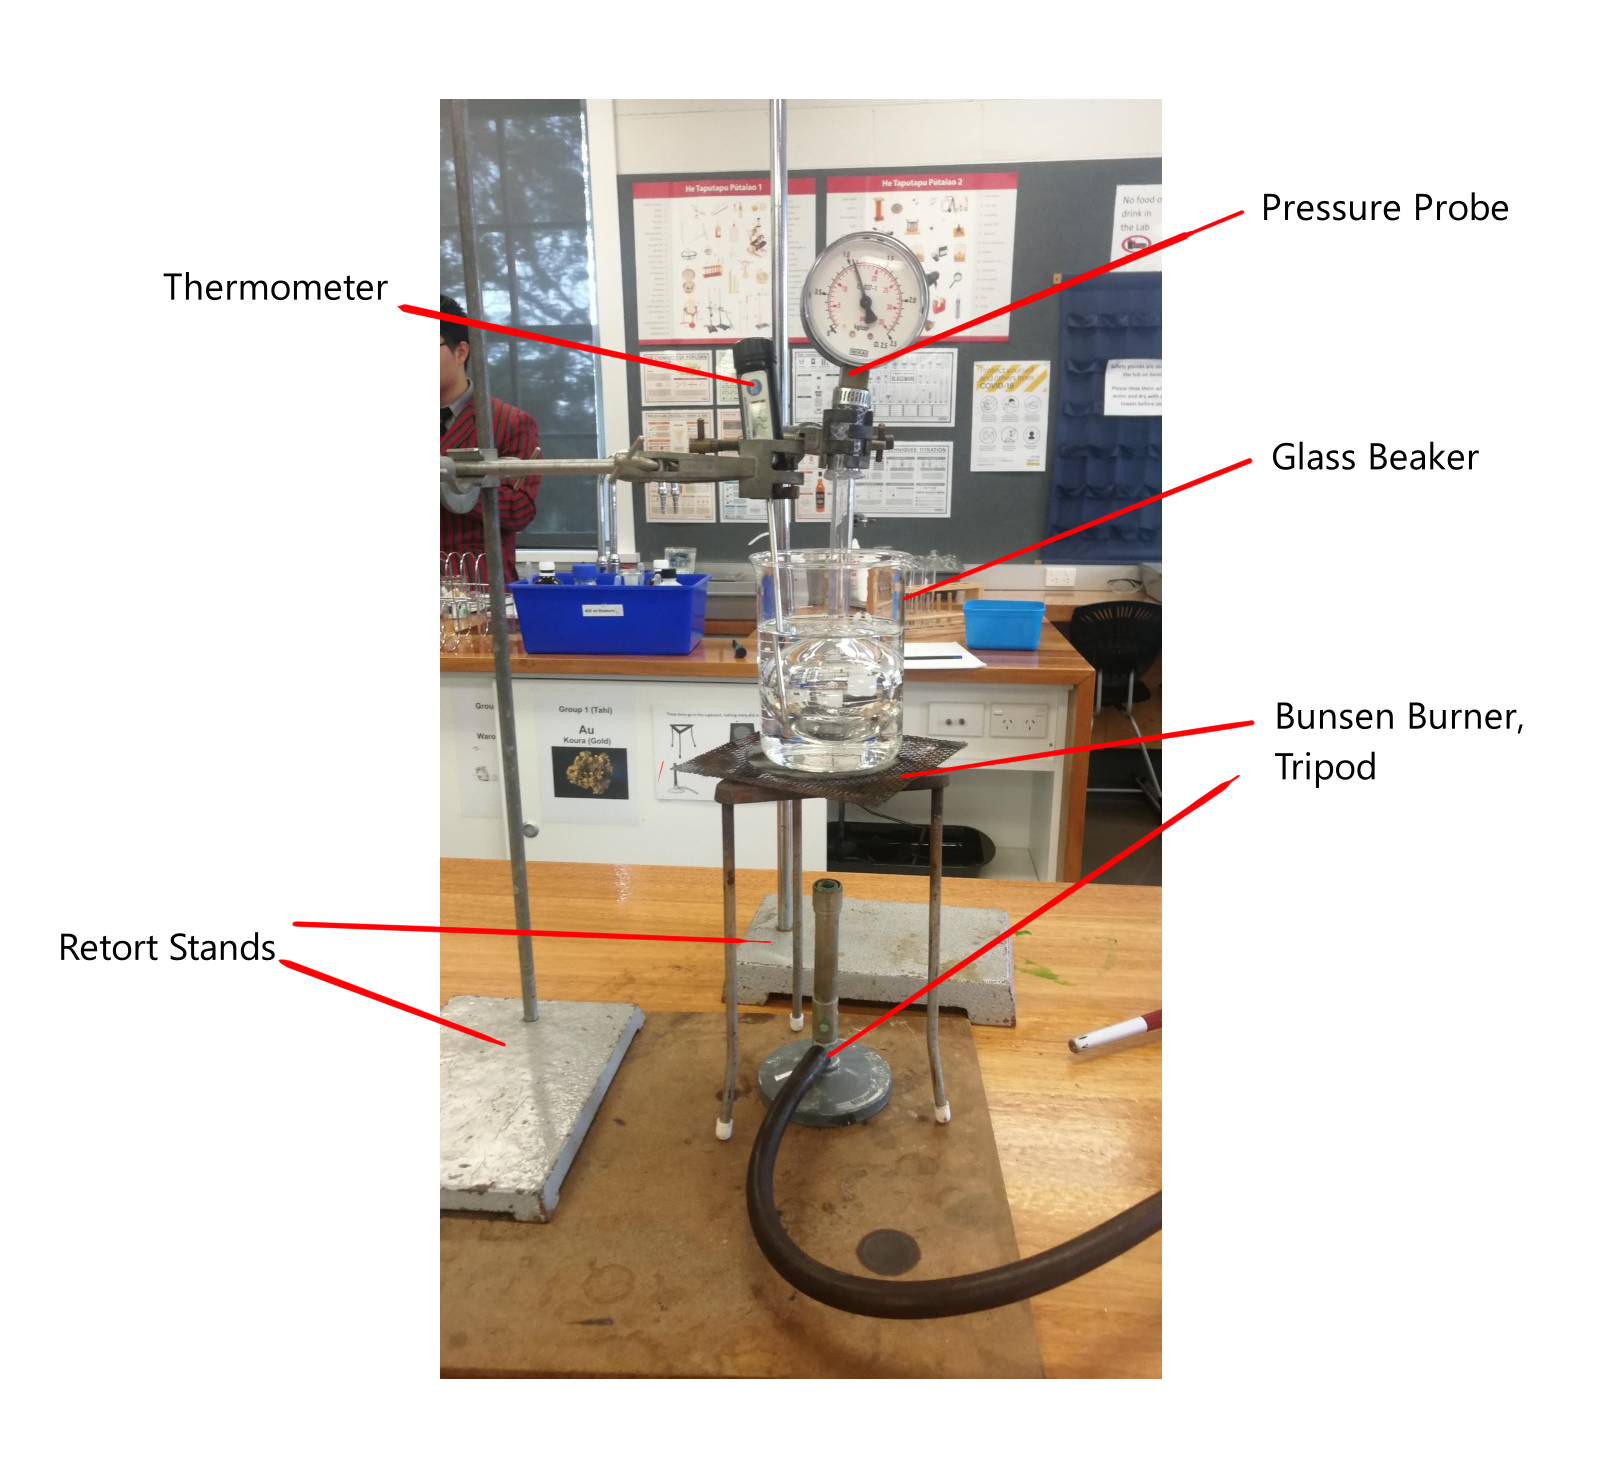
\includegraphics[width=\textwidth]{assets/setuplabelled.png}
    \captionof{figure}{The experiment setup, with the bunsen burner ready to be lit}
    \label{fig:setup}
\end{figure}

\begin{figure}[H]
    \centering
    \begin{minipage}{.4\textwidth}
        \centering
        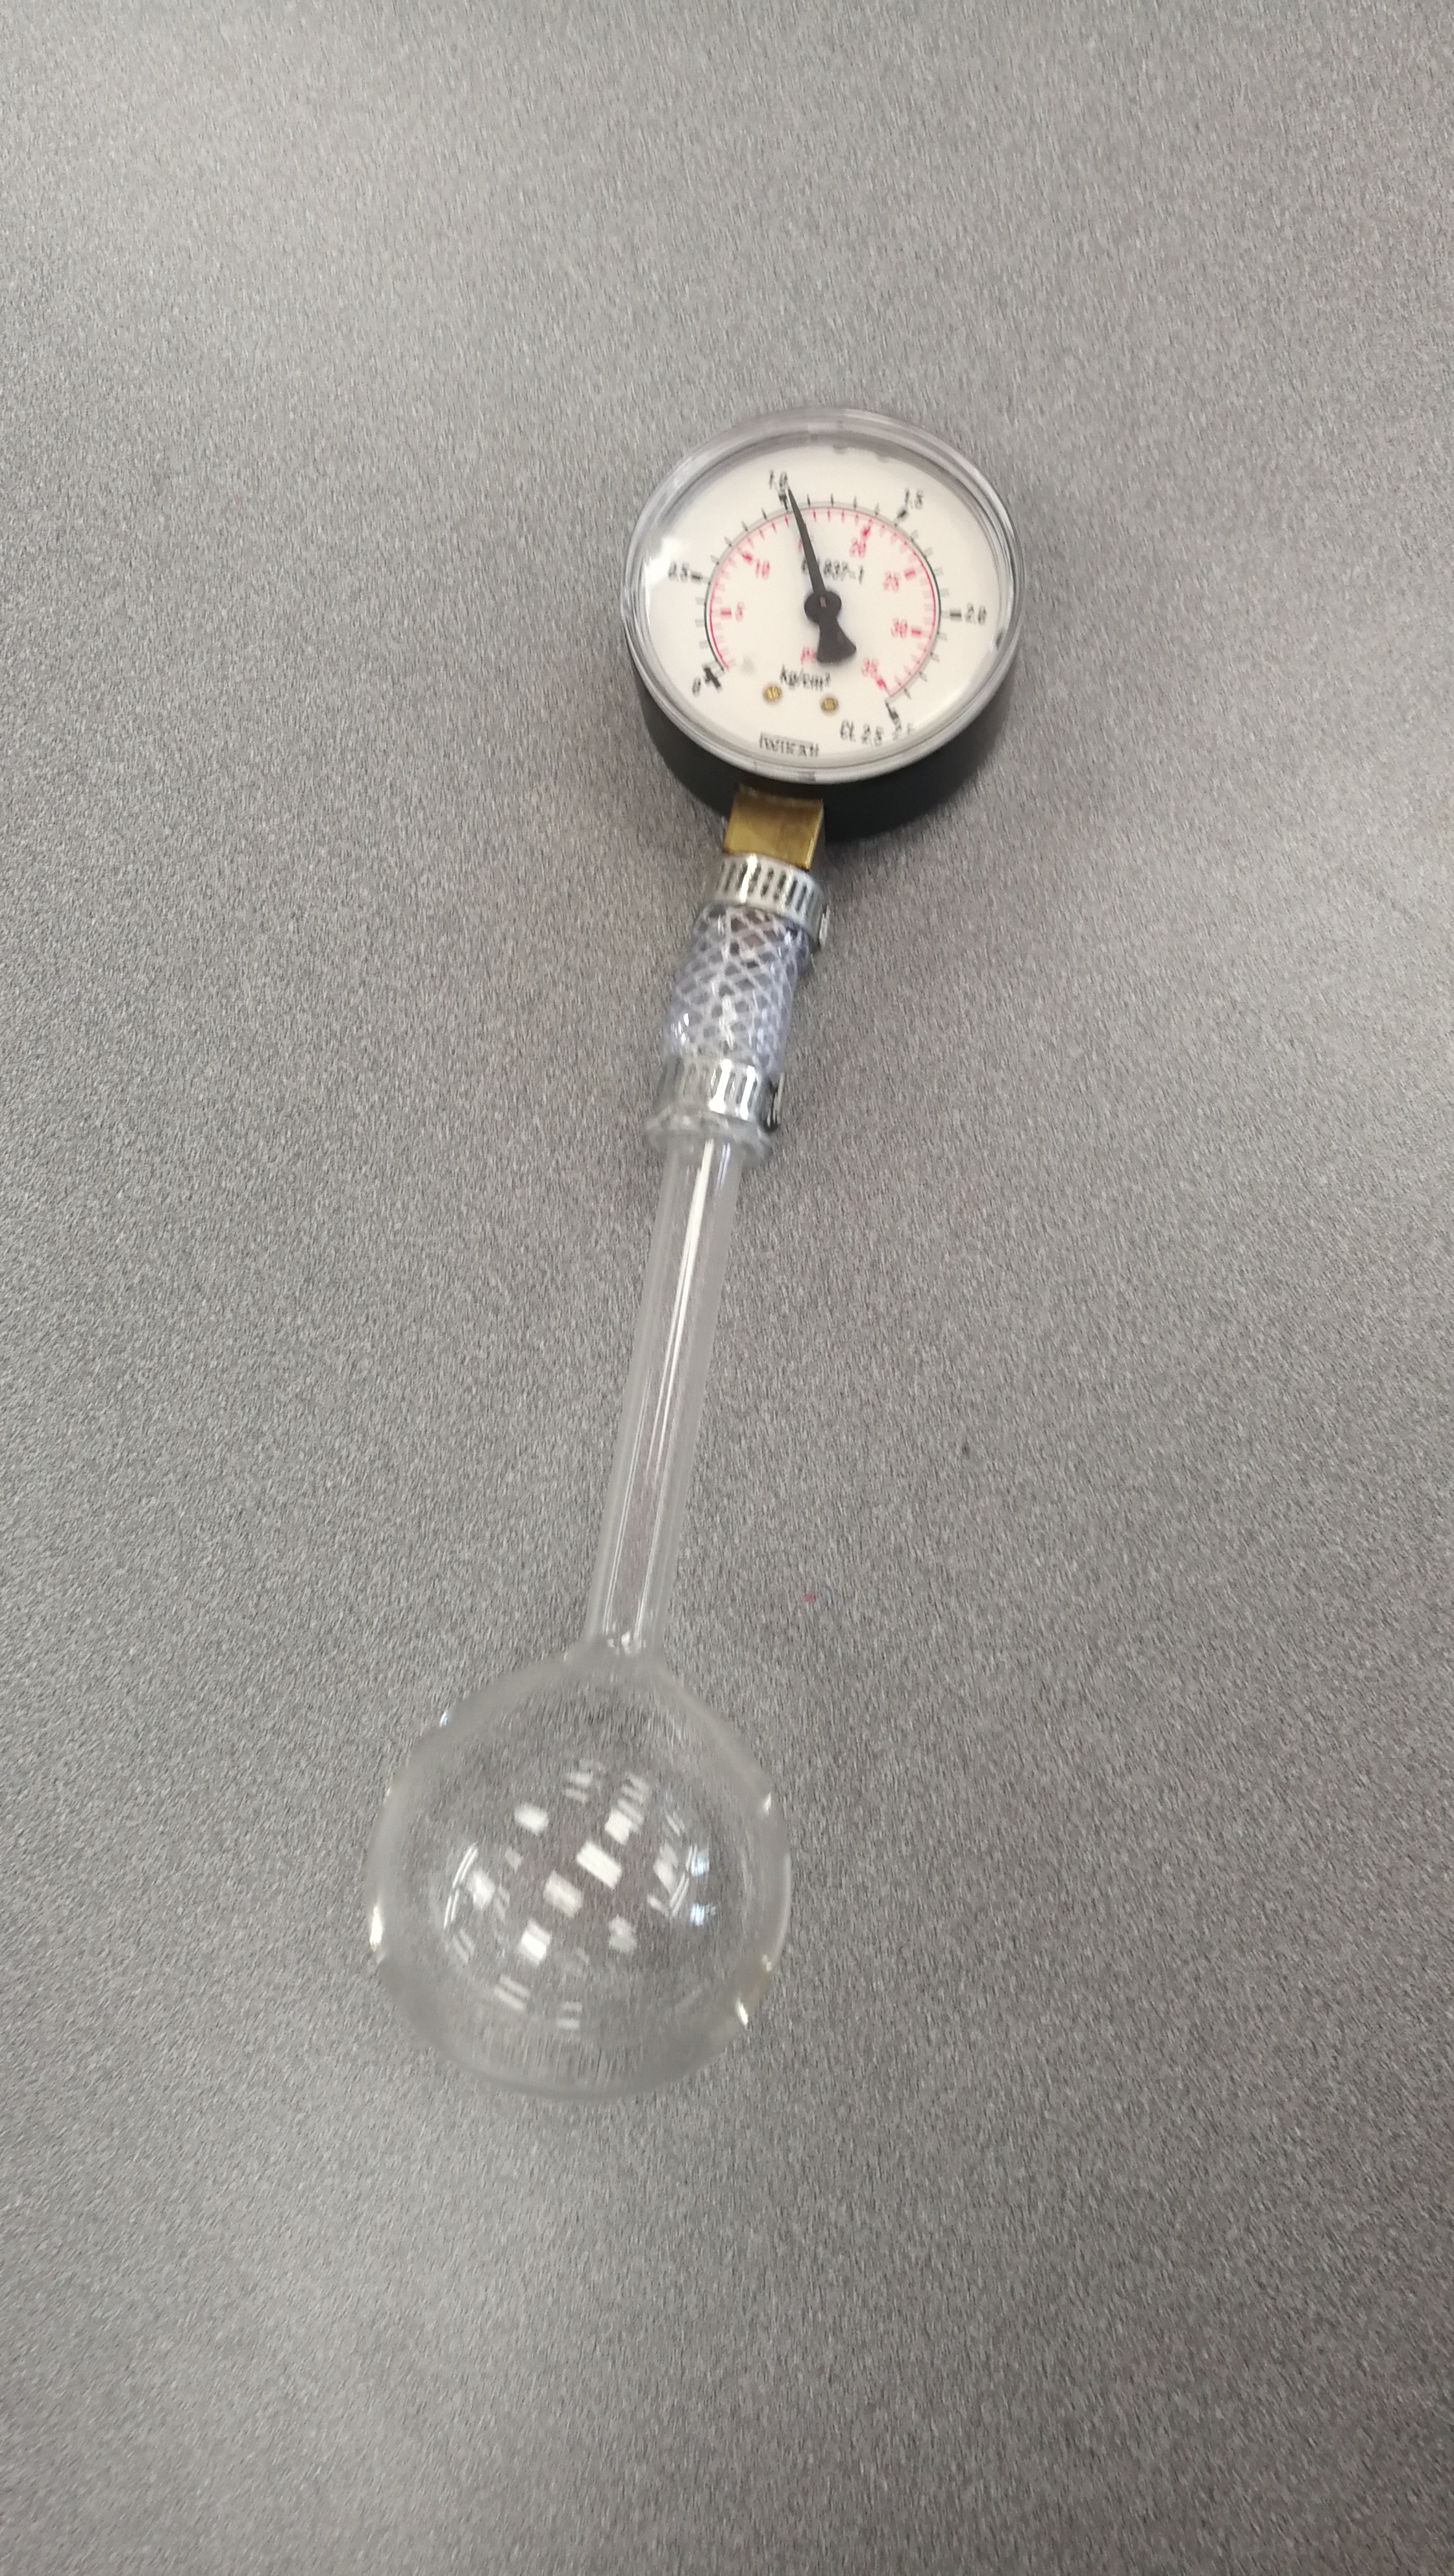
\includegraphics[scale=0.07]{assets/probe.jpg}
        \captionof{figure}{The gas pressure probe}
        \label{fig:probe}
    \end{minipage}%
    \begin{minipage}{.6\textwidth}
        \centering
        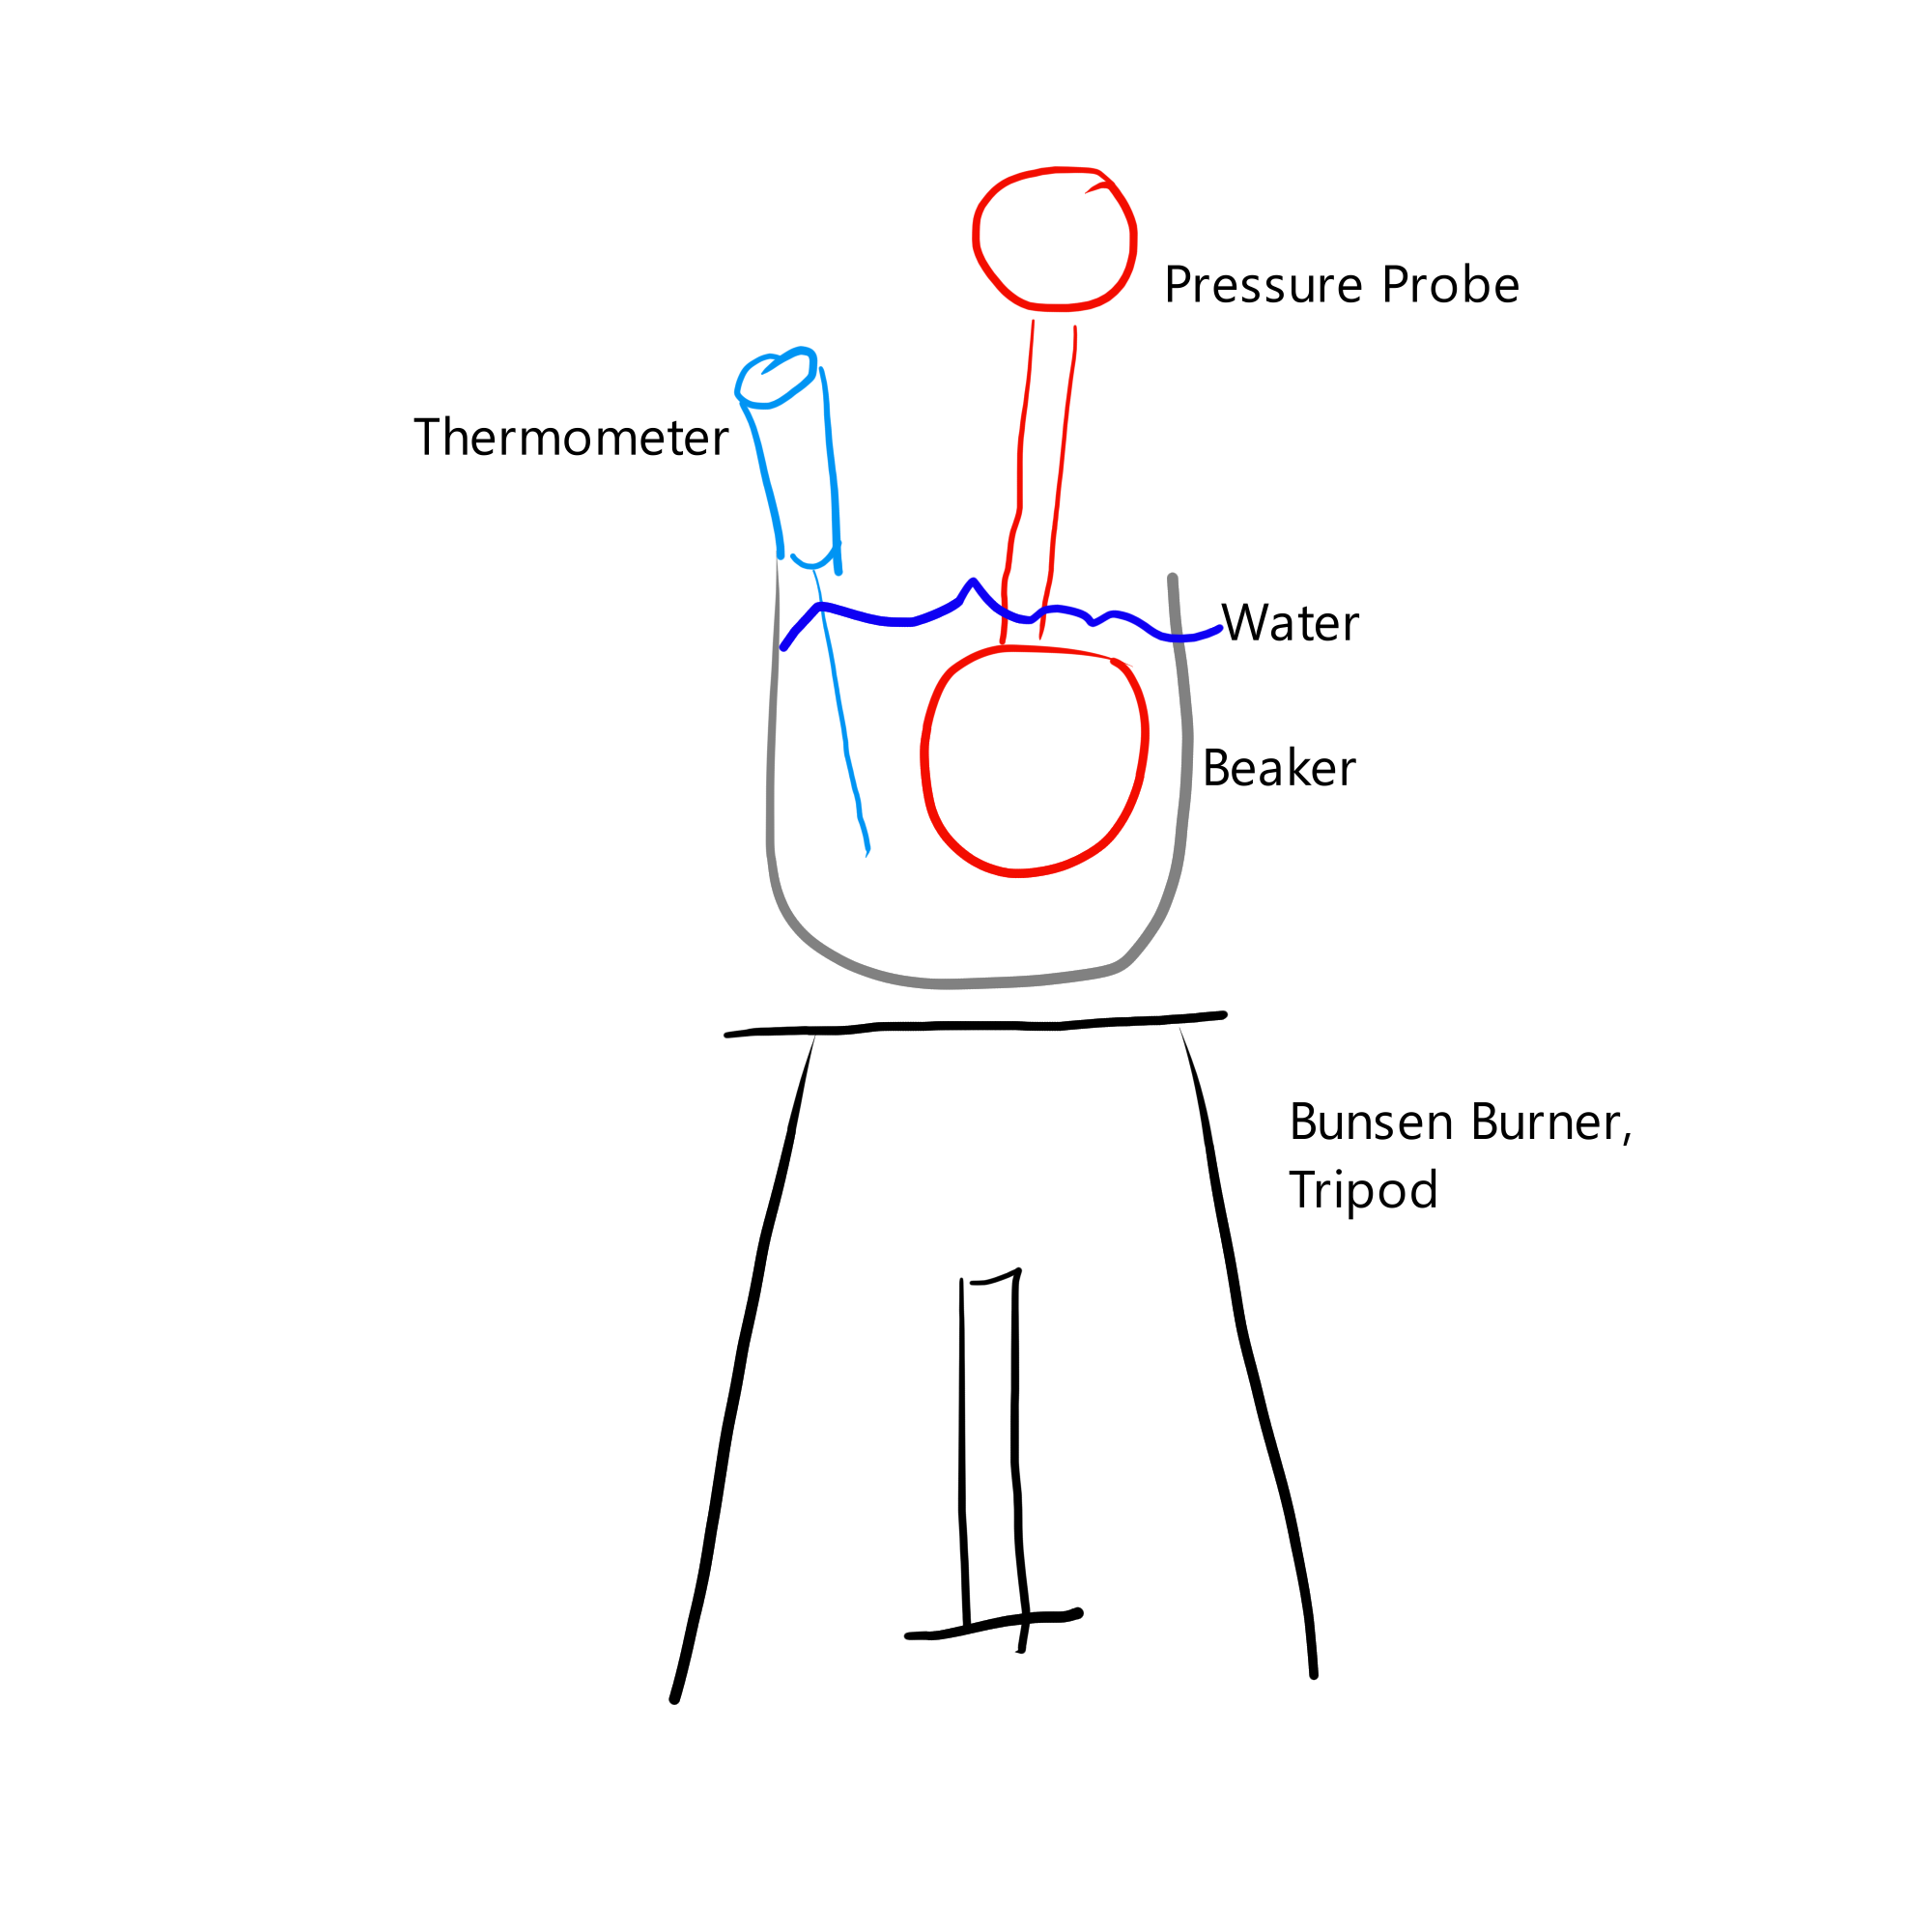
\includegraphics[scale=0.55]{assets/setupdrawn.png}
        \captionof{figure}{Sideview of the experiment setup}
        \label{fig:setupdrawn}
    \end{minipage}
\end{figure}

\subsection{Safety}
Working with pressure and high temperature presents a safety concern, wear eye protection throughout the experiment to protect against explosions.

Glass equipments are unstable during large temperature changes, care is needed in the handling of fragile glassware, wear close-toe shoes during the experiment and inspect the glassware between trials to protect against accidental leakages.

Take care in disposing hot water, for it can cause burns. Use a secondary beaker with cold water and slowing mix it with the primary beaker to cool it down.

\section{Data}
\subsection{Raw Data}
\subsubsection*{Qualitative data}
The endpoint of the heating is determined by the boiling point of water. In few trials, the intense boiling of the water started to shake the retort stands with the sensors, requiring me to end the experiment early in fear of the shaking resonating, causing spills.

The reason for a backup thermometer is because the high temperature of the water steamed up the display of the digital thermometer. I supposed operating with clamps at a dangerously high temperature is a potential safety hazard, therefore I stopped one of the trials from reaching temperatures higher than 75$\si{\celsius}$.

\subsubsection*{Quantitative data}
\begin{figure}[H]
    \centering
    \frame{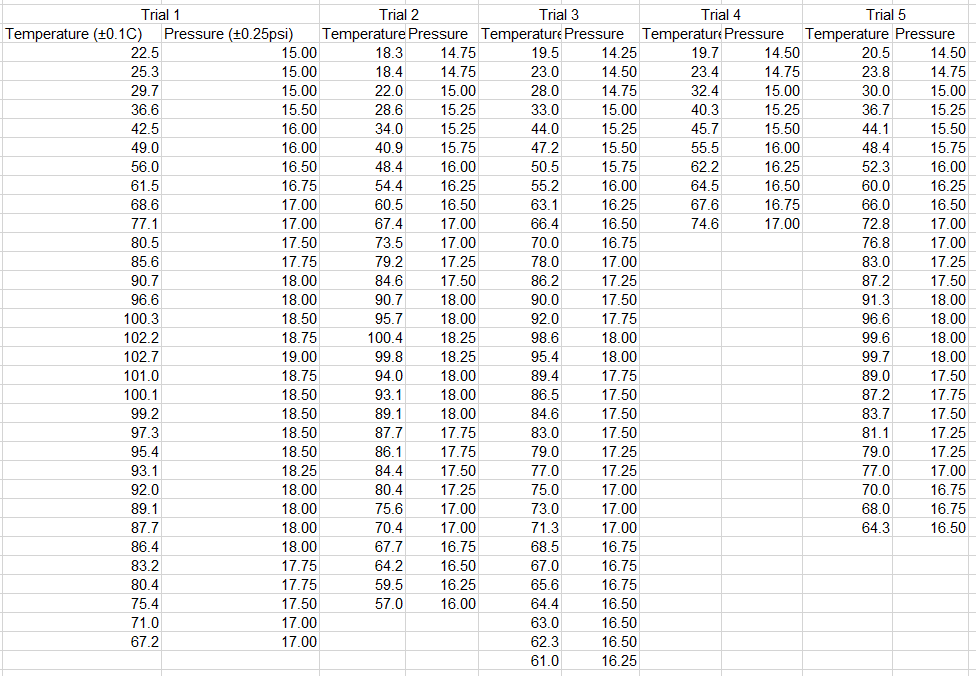
\includegraphics[width=\textwidth]{assets/rawdata.png}}
    \captionof{table}{Raw quantitiative data of 5 experiments, showing the relationship between pressure (kPa) against temperature ($\si{\celsius}$) of the air mixture}
\end{figure}

\subsection{Processing}
To convert between unit psi to kPa, the following conversion equation is used on all pressure measurements \parencite{conver_units}:
\[
    P_{\text{kPa}} \approx 6.89476 \times P_{\text{psi}}.
\]

\textit{Uncertainties}: $\relun P_{\text{kPa}} = \relun P_{\text{psi}}$

For example, in experiment 1, at temperature 22.5$\si{\celsius}$:

Pressure in kPa = 0.894757 $\times$ 15.00 $\approx$ $\num{1.034e+2}$,

$\absun P_{\text{psi}} = 0.25\si{psi}$

$\relun P_{\text{psi}} = \relun P_{\text{kPa}} =  \frac{0.25}{15.00} \approx 0.017$

$\absun P_{\text{kPa}} = 0.017 \times \num{1.0e+2} \approx \num{1.7} \si{kPa}$

Therefore: $P_{\text{kPa}} = \num{1.034e+2} \pm \num{1.7} \si{kPa}$

The full processed data tables are in the appendix: (table \ref{fig:pq}, table \ref{fig:upq}).

\newpage
\subsection{Analysis}

Transpose the pressure and temperature columns, the graph for experiment 1 is shown in figure \ref{fig:t1} --- the remaining graphs of the 4 additional experiments are in the appendix.

\begin{figure}[H]
    \centering
    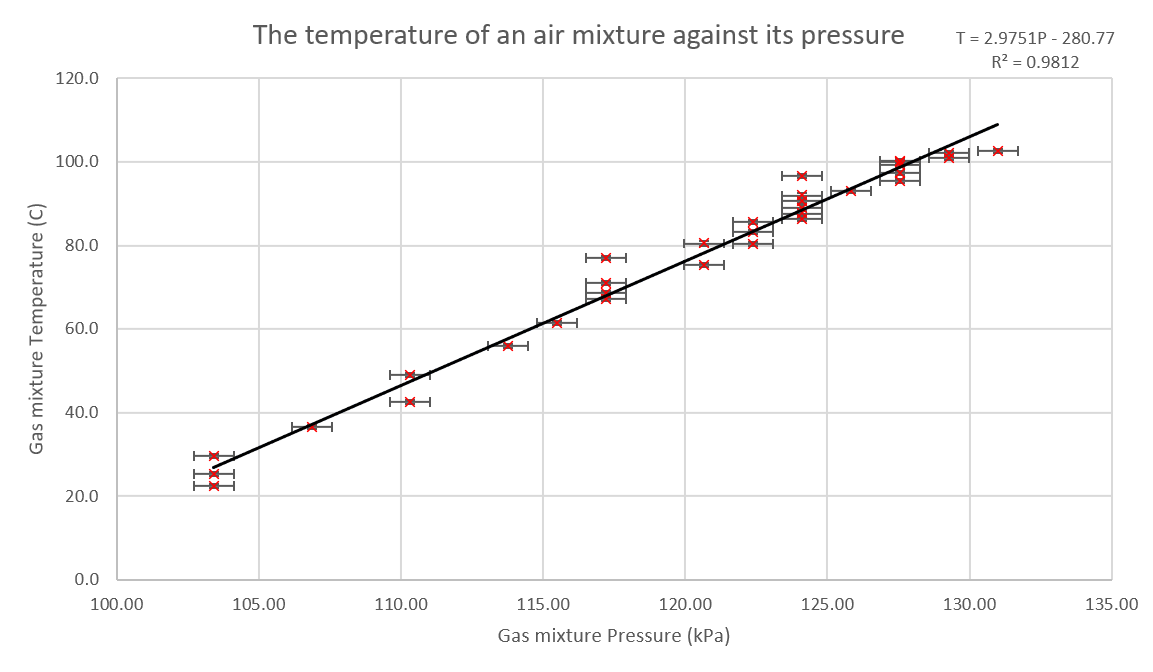
\includegraphics[width=\textwidth]{assets/graph1.png}
    \caption{Graph of the air mixture temperature against pressure for experiment 1}
    \label{fig:t1}
\end{figure}

\paragraph{Note} The y error bars shows the absolute uncertainties of the thermometer. The x error bars plots the calculated absolute uncertainties of the pressure measurements. The small uncertainty of the thermometer means the y error bars are not visible.

The value of absolute zero for each experiment is reflected in the y-intercept of their regression line. Averaging and calculating the half range for the 5 trials will increase the accuracy of the result (figure \ref{fig:yi}).

\begin{figure}[H]
    \centering
    \frame{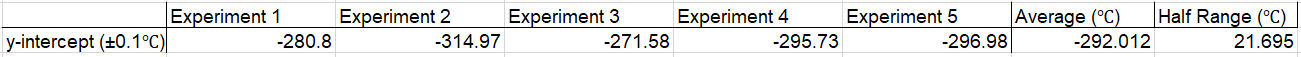
\includegraphics[scale=0.45]{assets/azerodata.png}}
    \captionof{table}{The y-intercepts of the experiments}
    \label{fig:yi}
\end{figure}


Average of the y-intercepts: $\frac{\sum \text{y-intercepts}}{5} \approx -292.0 \si{\celsius}$

Half range of the y-intercepts: $\frac{\max - \min}{2} \approx 21.70 \si{\celsius}$

Therefore, our empirical value for absolute zero is: $-290 \pm 20 \si{\celsius}$

The International System of Units defines the absolute zero at $-273.15\si{\celsius}$ \parencite{si_form}, which is within our uncertainty region: \[-310 < -273.15 < -270\] The percentage error of the our empirical value is: $\frac{-273.15- -290}{-273.15} \approx 6.16\%$

However, I was curious and thought to use another method to compute the absolute zero using the given dataset. By combining the data from all of the experiment into one dataset, the result can be graphed and a regression line can be fitted (figure \ref{fig:comb}). I believe that this method will result in a more realistic value and uncertainty, given that it is analogous to conducting a really long experiment with multiple cooling and heating steps.

\begin{figure}[H]
    \centering
    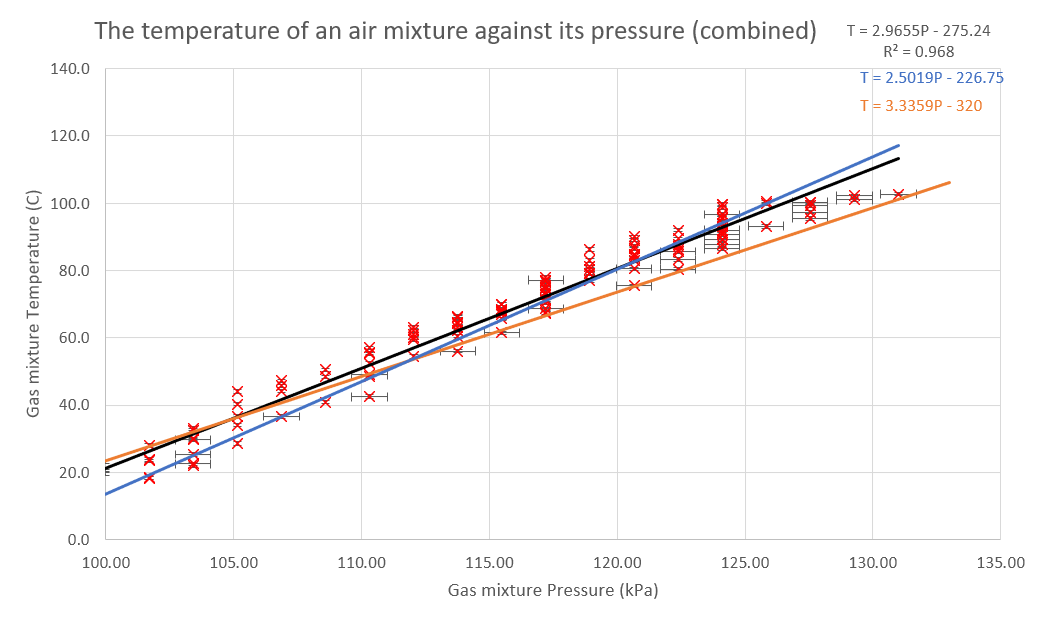
\includegraphics[width=\textwidth]{assets/combinedgraph.png}
    \caption{Data graph for the combination of datasets}
    \label{fig:comb}
\end{figure}

Using this method, the measurement of absolute zero is the value of the y-intercept of line of best fit. The uncertainty can be calculated using the half range between the Most Sloped line of worst fit (MSLWF) and the Least Sloped line of worst fit (LSLWF).

y-intercept = $-275.2\si{\celsius}$

MSLWF = $-214.5\si{\celsius}$, LSLWF = $-320.0\si{\celsius}$

\textit{Uncertainty}: $\frac{\text{MSLWF} - \text{LSLWF}}{2} \approx 52.8 \si{\celsius}$

Therefore, the experimental value of absolute zero using this method is: $-270 \pm 50 \si{\celsius}$. The percentage error is: $\frac{-270 - -273.15}{-273.15} \approx 1.15\%$

\section{Conclusions}
\subsection{Result}
There exists a clear and strong positive correlation between the temperature and pressure of the air mixture, as shown in the positive sloping regression line in figure \ref{fig:t1}, and the close to one correlation coefficients. This shows that as the pressure of a gas increases, the temperature will also increase, and vice versa.

% uncertainty
In both methods, there are some rather largely sized error bars in the pressure measurements. This is caused by the large uncertainties of the pressure probe, for its scales have large gaps. This contributed in decreasing the precision of the resultant value of absolute zero.
% accuracy and % error
The value and range of absolute zero computed in both methods contain the true value of absolute zero, signifying the success of the method. The low percentage error of 6.16\% and 1.15\% for both methods displays the high accuracy of the data. Additionally, this suggests that the usage of multiple trials had succeeded in improving the accuracy of the outcome. The experiment data is considered to be highly accurate but less precise.

% theory & science involved
The high correlation coefficients in both methods showcase a strong correlation between the temperature and pressure of a gas mixture at constant volume and amount. Additionally, there were no anomalous results in the 5 trials even when the data is being collected on separate days and times. This strongly confirms my hypothesis of the relationship between gas temperature and pressure, where it is described as:
\[
    T = kP + T_{\text{absolute zero}},
\]

and $k$ is the proportionality constant. This confirms a part of the ideal gas law (figure \ref{fig:igl}), and showcases the validity of the kinetic theory of ideal gases.
%
By assuming the air mixture in the pressure probe as an ideal gas: the most important assumptions here are that the volume and intermolecular forces of the particles are negligible. Because pressure is a measure of the average collision force per area from the particles against the glass spherical container, increasing temperature will increase the average kinetic energy of the particles within the glass container, which increases the speed of these collisions, creating higher pressure.

\subsection{Implications}
The obvious implication of the relationship between temperature and pressure is to offer a very simple procedure to measure the value of absolute zero. For past scientists, this value is the uttermost important piece of the puzzle that is in the creation of the gas kinetic theory, because a non-standardized unit of temperature will be plagued with minus signs at certain conditions, which increases the complexity of the formulas.

% maybe talk about the implications of the relationship, boiling & melting points, propane gas cans and atlitudes.
% but already too much words
\subsection{Evaluation}

%Here is a list on the handling of the controlled variables/potential error factors, and future improvements to be made.

\subsubsection{Random Errors}
\paragraph{Large uncertainties of the pressure probe} This is very significant in contributing to the lack of precision in the dataset. The large size of the steps (0.25$\si{psi}$) in the scales and the small range of changes in the pressure relative to the scale means that a sizable temperature change may not cause a visible pressure change, leading me to note down the same value twice or more, thus increasing the spread of the data points. I have attempted to counteract this by using a timer and a constant interval, but a more precise measurement is required, I suggest increasing the range of pressure measurements --- starting with cold water instead of at room temperature, and using a less uncertain instrument.

\paragraph{Malfunctions of the thermometer}
May be significant in reducing precision of high temperature readings. The digital thermometer's readings fails to display at high temperatures, leading me to guess an approximate value. This is partial handled by switching to a new thermometer when the current one fails. Also consider conducting the experiment at relatively lower light levels to ease the temperature readings; or to create a plastic shield placed under the head of the thermometer.

\paragraph{Delay in data readings}
Slightly significant in increasing the spread of the dataset. The separate recording of the two sensors means that there is a random variable of delay between the temperature and pressure readings. Consider using a data logger instead of human judgment.

\subsubsection{Systematic Errors}
\paragraph{Boiling of the water}
Relating to the controlled variable of the volume of water in the beaker, a fear of mine is that the boiling of the water will systematically shift the pressure measurements at higher temperatures upwards. The vaporization of water creates water vapor with a temperature higher than $100\si{\celsius}$, heating the stem of the pressure probe and causing a systematic difference in the temperature of the air mixture and water. This is likely to explain the dip in the transposed Temperature/Pressure graph in figure \ref{fig:comb}. Consider stopping the heating process at around $90-95\si{\celsius}$ to increase the accuracy of the result.

\paragraph{Environmental temperatures}
Less significant in decreasing the accuracy of the \\result. For the stem of the pressure probe is not submerged into water, a colder room temperature will systematically increase the water and air mixture temperature difference, particularly at lower temperatures. But the variable controlled in the experiment and no significant systematic shifts at lower temperatures are seen.

\paragraph{Delay in heat transfer}
The method relies on the conduction heat transfer between the water to the air mixture across glass. A systematic temperature difference in temperature may decrease the accuracy of the data points throughout all temperatures, but the low \% error indicates a low significance of this error.

\paragraph{Sensors}
In a few trials, the temperature readings as the water boils are seen to increase above $100\si{\celsius}$. This showcases the systematic error of the thermometer, which shifts all points upwards in the transposed graph, resulting in a higher point of absolute zero. However, this is not the case in the experiment, which can be explained through the likely influence of the dipped higher pressure points, overwriting the systematic errors of the temperature sensor. Consider using an additional mercury thermometer alone side the digit one, and average their measurements to increase the accuracy of the final result of absolute zero.

\subsection{Further Investigations}
To further investigate the ideal gas law and the value of absolute zero, other relations from the equation (figure \ref{fig:igl}) can be used. One can measure the volume of an air mixture against its temperature using an ice bath and a freely moving syringe with air inside. The y-intercept of the volume against temperature graph will be the value of absolute zero as well. This may give a more certain estimation of absolute zero, for the volume readings on syringes may be less uncertain than the pressure probe.

Furthermore, an interesting experiment would be to test the deviation of the ideal gas law at low temperatures or high pressure. By performing the aforementioned experiments in a freezer or on top of a mountain, it is likely to explain and correct the small but significant systematic errors in this experiment.

\newpage
\nocite{*}
\printbibliography


\newpage
\section*{Appendix}
\appendix
\begin{figure}[H]
    \centering
    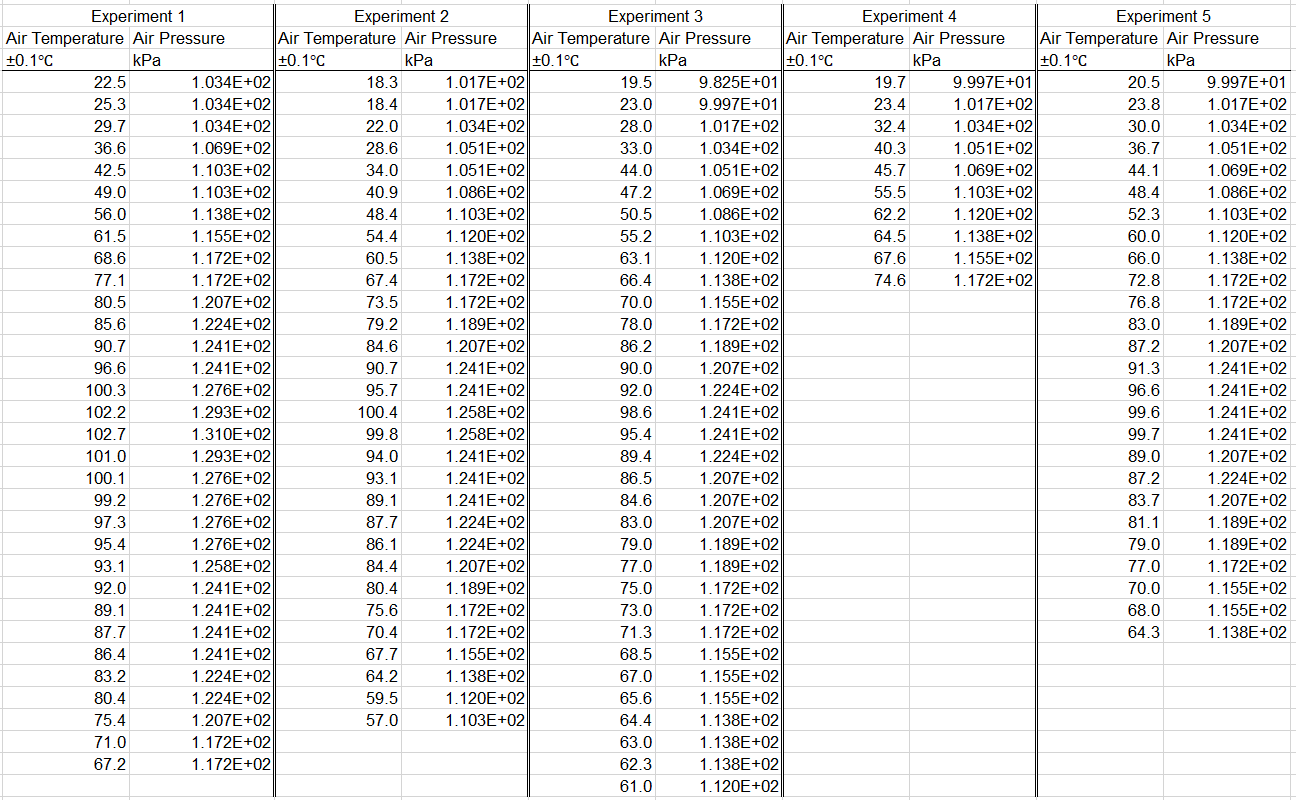
\includegraphics[width=\textwidth]{assets/unitdata.png}
    \captionof{table}{Processed quantitivative data of 5 experiments, showing the relationship between pressure (kPa) against temperature ($\si{\celsius}$) of the air mixture}
    \label{fig:pq}
\end{figure}

\begin{figure}[H]
    \centering
    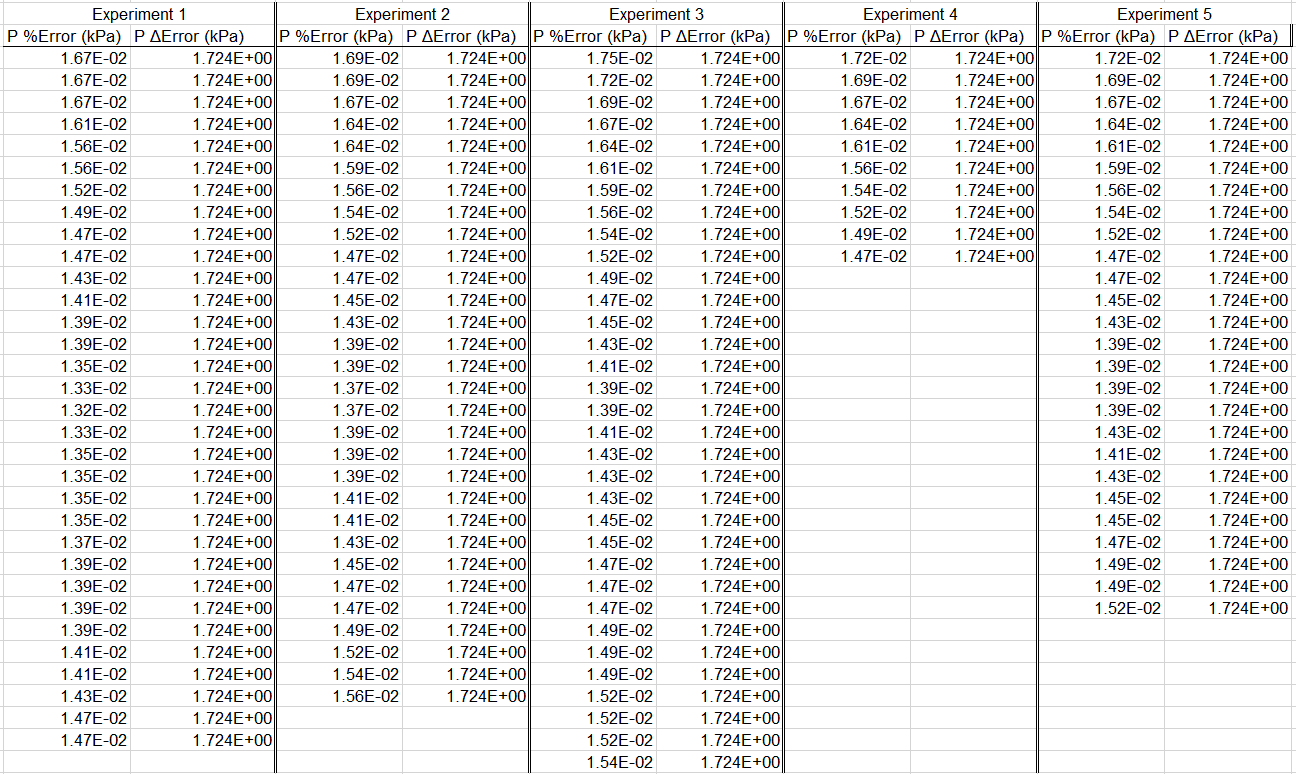
\includegraphics[width=\textwidth]{assets/unitdata_unc.png}
    \captionof{table}{Uncertainty of the processed quantitivative data of 5 experiments}
    \label{fig:upq}
\end{figure}


\begin{figure}[H]
    \centering
    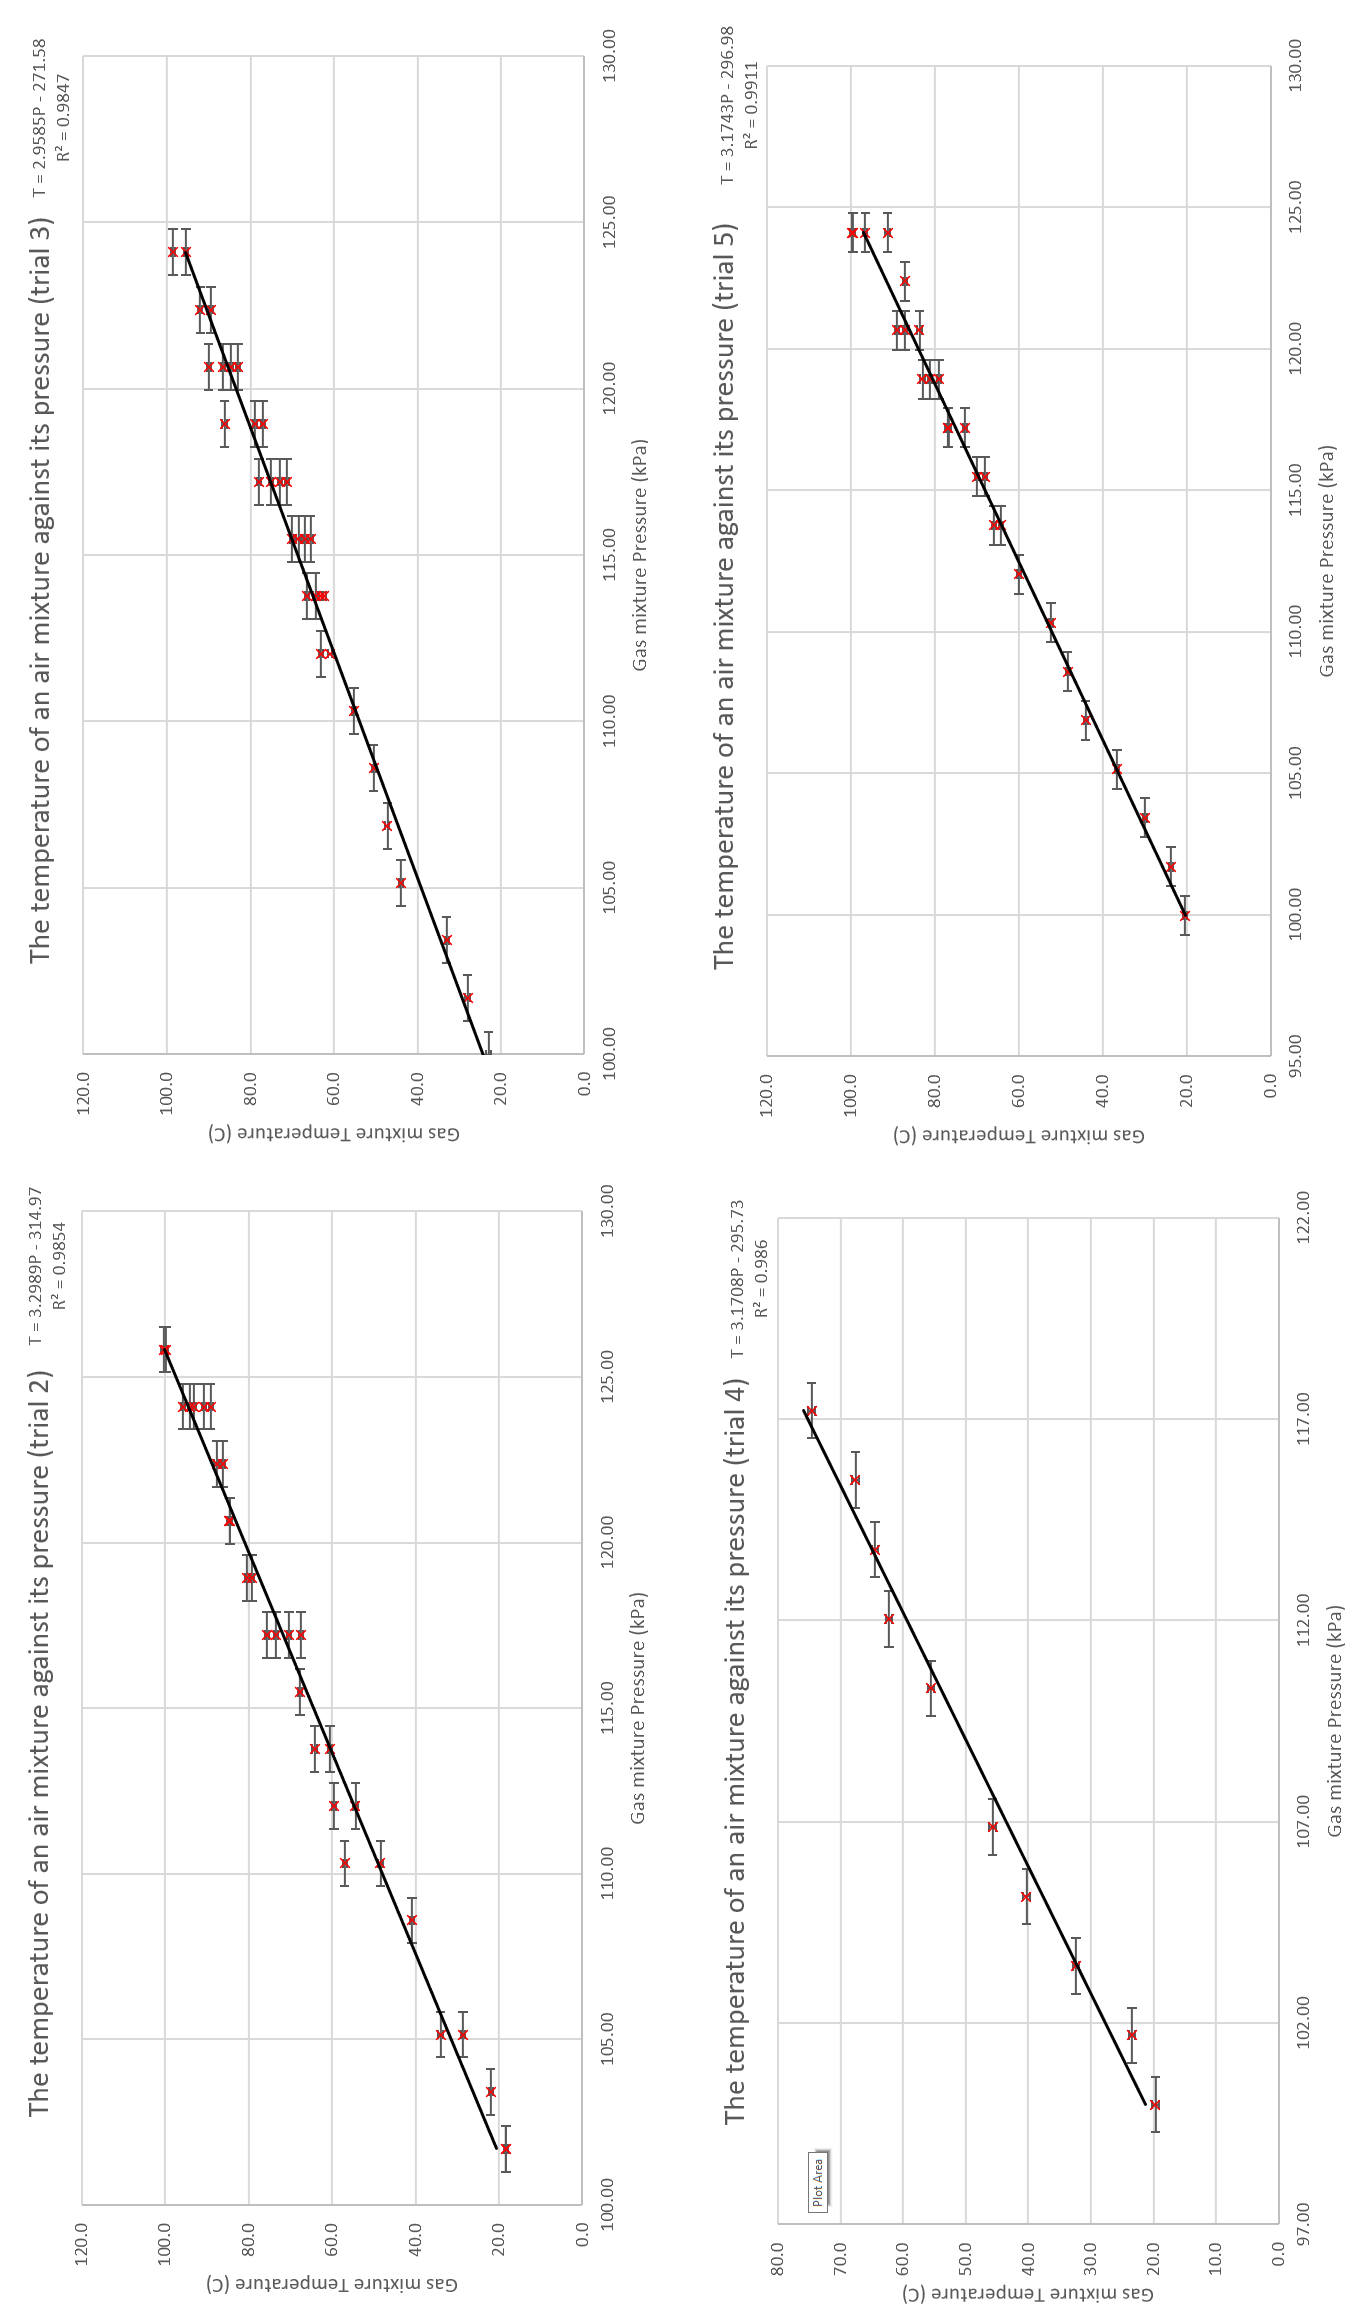
\includegraphics[width=0.76\textwidth]{assets/graphs.png}
    \captionof{figure}{Data graphs of trials 2-5}
    \label{fig:dg25}
\end{figure}

\end{document}
